%%%%%%%%%%%%%%%%%%%%%%%%%%%%%%%%%%%%%%%%%
% University/School Laboratory Report
% LaTeX Template
% Version 3.1 (25/3/14)
%
% This template has been downloaded from:
% http://www.LaTeXTemplates.com
%
% Original author:
% Linux and Unix Users Group at Virginia Tech Wiki 
% (https://vtluug.org/wiki/Example_LaTeX_chem_lab_report)
%
% License:
% CC BY-NC-SA 3.0 (http://creativecommons.org/licenses/by-nc-sa/3.0/)
%
%%%%%%%%%%%%%%%%%%%%%%%%%%%%%%%%%%%%%%%%%

%----------------------------------------------------------------------------------------
%	PACKAGES AND DOCUMENT CONFIGURATIONS
%----------------------------------------------------------------------------------------

\documentclass{article}

\usepackage[version=3]{mhchem} % Package for chemical equation typesetting
\usepackage{siunitx} % Provides the \SI{}{} and \si{} command for typesetting SI units
\usepackage{graphicx} % Required for the inclusion of images
\usepackage{natbib} % Required to change bibliography style to APA
\usepackage{amsmath} % Required for some math elements 
\usepackage{listings} % For my generic code input
\usepackage{color}
\definecolor{deepblue}{rgb}{0,0,0.5}
\definecolor{deepred}{rgb}{0.6,0,0}
\definecolor{deepgreen}{rgb}{0,0.5,0}

\usepackage{listings}
\lstset{language=Python}

\usepackage[a4paper, total={6in, 8in}]{geometry}

\setlength\parindent{0pt} % Removes all indentation from paragraphs

\renewcommand{\labelenumi}{\alph{enumi}.} % Make numbering in the enumerate environment by letter rather than number (e.g. section 6)

%\usepackage{times} % Uncomment to use the Times New Roman font

%----------------------------------------------------------------------------------------
%	DOCUMENT INFORMATION
%----------------------------------------------------------------------------------------

\title{CWI User Manual} % Title

\author{Reuben \textsc{Zotz-wilson}} % Author name

\date{\today} % Date for the report

\begin{document}

\maketitle % Insert the title, author and date

\begin{center}
\begin{tabular}{l r}
Date updated: & 22 July, 2016 \\ % Date the experiment was performed
Partners: & Thijs Boerrigter \\ % Partner names
\end{tabular}
\end{center}

% If you wish to include an abstract, uncomment the lines below
% \begin{abstract}
% Abstract text
% \end{abstract}

%----------------------------------------------------------------------------------------
%	SECTION 1
%----------------------------------------------------------------------------------------

\section{Introduction}

This manual describes the use of a package of functions which allow the processing of time series data for the purpose of coda wave analysis. The initial intention was to expedite the analysis of time lapse, ultrasonic data acquired during axial loading experiments. The processing is now generalised to allow in input of two basic data streams, time-series (TS) data and any number of complementary perturbation vectors.
 
%----------------------------------------------------------------------------------------
%	SECTION 2
%----------------------------------------------------------------------------------------

\section{Data Input}
Two principal data types are taken as input, the time series (e.g. Ultrasonic time lapse traces) and the corresponding perturbation dataset (e.g. axial loading information). The following will detail the accepted input formats for these two principal data streams. The raw input data will be loaded into memory and then saved to disk in a HDF5 database. 

Note: I need to generalise the input data further, and instead of searching for the format, simply ask the user to specify the input data format types. 

\subsection{Binary TS Data and CSV PV Data}
The user must provide a folder containing binary file TS data only, along with a single csv file all PV data formats. (This import function needs to be generalised)

\subsection{Database loading}
After the first run of a particular dataset a folder \texttt{"TS\_loc"\_DB} will be created in the run folder. A HDF5 database \texttt{TS\_raw\.h5} will be created containing a single table titled \texttt{TS\_full}. Due to the shape of such time series information, typically square instead of tall this database is saved in "fixed" format and therefore can not be queried. Another database \texttt{DB\_tbl\.h5} will be also created at this point in the same folder, containing the remaining imported data, this dataset can be queried.   \newline.

\begin{tabular}{l|p{120mm}}
\texttt{TS\_raw\.h5} & hdf5 database containing all TS data within the input folder\\
\texttt{TS\_full} & Tabel name stored within \texttt{TS\_raw\.h5}\\
\texttt{DB\_tbl\.h5} & hdf5 database containing all input PV and TShdrs data found \\
\end{tabular}
\newline

If the user input parameter \texttt{loadDB} is set to \texttt{True} and existing \texttt{DB\_tbl\.h5} and \texttt{DB\_tbl\.h5} databases are found within the folder \texttt{TS\_loc\_DB}, then no reload of the raw input data will be performed. Instead, the hdf5 databases will be loaded, after which all normal processing is possible. Note, it is preferable to avoid re-loading any initial data formats as this step is time consuming, particularly for large numbers of CSV files. \newline

After the processing is finished, \texttt{run\_datastore()} will be called. This function within the class \texttt{dataStore} will create the following databases within the folder \texttt{"TS\_loc"\_DB} . \newline

\begin{tabular}{l|p{120mm}}
\texttt{DB\_tbl\_processed\.h5} & hdf5 database containing the processed PV and CC and TShdrs\\
\texttt{TS\_cut\.h5} & hdf5 database containing the TS data equal to the number of CC rows. The table name \texttt{TS\_df} can be used to access the this table. Note: this databased is saved in "fixed" format and therefore cannot be queried\\
\end{tabular}
\newline

\subsection{section}

\subsection{Time Series}
The accepted formats for the time series (TS) data are ".CSV" and binary file formats. In both cases a single file is expected to contain a vector of amplitude with a constant sampling frequency. If multiple receivers are available for each measurement step stored within the same file, the user must select which receiver is to be analysed. File numbering should increase with the time of measurement, where the date and time of the file creation is used to match the TS data to its corresponding PV (perturbation vector - time column).

\subsection{Perturbation Vectors}
The perturbation vectors are input from a ".CSV" file, where the display of both a primary and secondary vector is possible. The primary data is intended to be plotted against the CWI CC's (Cross-correlation Coefficients) when the perturbation is in a continuous direction. In the case of a cyclic perturbation measurement numbers or measurement time should be input as the primary perturbation vector. The secondary perturbation vector is intended to be used for line of surface colouring, in order to display this data on the same plot as the CC's. 

\subsection{Paramater Setup File}
Parameter input and overall control of the signal processing is handled by an input text file. There are two types of inputs, those which are mandatory such as the relative folder location for the TS data, and those which have a default value if not defined, such as the sample or run name. An example of the input syntax is given below:


\begin{lstlisting}[basicstyle=\small]
% input file for python based CWI processing
FB_cut = 1 % sample points to remove from all TS traces
END_cut = 5000 % sample point after which all will be removed from all TS traces
STA_meas = 1 % start of TS measurements included in processing
END_meas = 10 % last measurement to be included in processing


% Cross-correlation parameters
ww = 400 % the window with in number of samples
ww_ol = 10 % the window with [%] overlap
CC_ref = 1 % If one is selected 


\end{lstlisting}


\subsection{User input variable description List}
\begin{tabular}{l|p{120mm}}
\texttt{import\_dtype} & The date type to import, Either 'bin\_par', 'Shell\_format' or 'NoTShdrer\_format'. Default is  'bin\_par'\\
\texttt{TSloc} & location of time series data containing folder or single file\\
\texttt{PVloc} & location of pert. data containing folder or single file\\
\texttt{loadDB} & True or False, any existing raw database file will be loaded in place of the raw input data formats.\\
\texttt{acqDate} & The date of acquisition, is required for some data types which are not time matched \\
\texttt{recNo} & The receiver number which will be selected for processing, if not given no TS splitting will be attempted\\
\texttt{sampNo} & The number of sample points in a single trace recording, only required as input if the rec\\
\texttt{SampFreq} & The number of samples recorded per second\\
\end{tabular}
\newline

Pree-processing inputs\newline
\begin{tabular}{l|p{120mm}}
\texttt{stress\_strain} & If "True", an attempt will be made to calculate stress and strain from inputs L and D assuming a cylinder\\
\texttt{L} & The length of sample in mm\\
\texttt{D} & The diameter of the sample in mm\\
\texttt{Ax\_Press\_corr\_ADT} & [micron/bar] correction for depletion strain calculation\\
\texttt{Rad\_press\_corr\_ADT} & [micron/bar] correction for depletion strain calculation\\
\texttt{avg\_Press\_corr\_RDT} & [micron/bar] correction for depletion strain calculation\\
\texttt{Temp\_corr} & [micron/DegC] correction for depletion strain calculation\\
\texttt{Pax\_friction} & correction for depletion strain calculation\\
\texttt{LVDT\_zidx} & Index point in perturbation data frame where LDVT will be zeroed\\
\texttt{LLLength} & Length in sample points of the Linear Line, if given the search for the most linear line will run. Note: 'Stress [MPa]' and 'Strain Ax. [\%]' must be in PV\_df\\
\texttt{FB\_cut} & Number of sample points to remove from the start of each TS\\
\texttt{END\_cut} & Sample point after which all following will be removed\\
\texttt{STA\_meas} & The first measurement to be included in the processing\\
\texttt{END\_meas} & The last measurement to be included in the processing\\
\texttt{PV\_STA} & The first PV measurement to include in display of information\\
\texttt{PV\_END} & The last PV measurement to include in display of information\\
\texttt{TS\_samp\_dt} & The TS sampling dt in seconds. If given then time matching will be based on both the dt and the first .par file count vector.\\
\texttt{match\_timeshift} & Time shift to the TS file acquisition time in seconds. Only used in conjunction with \texttt{TS\_samp\_dt}.\\
\texttt{TS\_file\_tmatch} & Match TS data based on time file last modified.\\
\end{tabular}
\newline

Cross-Correlation parameters\newline
\begin{tabular}{l|p{120mm}}
\texttt{ww} & The correlation window width in sample points. If  \texttt{wdwPos} is given then \texttt{ww\_ol} is irrelevant and \texttt{ww} must have the same number of entries as \texttt{wdwPos}\\
\texttt{ww\_ol} & The percentage overlap of windows\\
\texttt{wdwPos} & The select positions of correlation windows in sample points\\
\texttt{CC\_type} & Either 'fixed' or 'rolling' to define the CC type input\\
\texttt{CC\_ref} & 1,2,3...etc TS as fixed or rolling reference\\
\texttt{Eng\_ref} & If True, and \texttt{CC\_type}='rolling', energy comparison will be made with the first TS acquired. If False, comparisons will be made with same TS as CC.  \\
\texttt{taper} & Either 'True' or 'False' to filter with a hann window each CC window. Note the default is set to False if taper not given in the input file.\\
\end{tabular}
\newline

Post Processing Paramerters\newline
\begin{tabular}{l|p{120mm}}
\texttt{FBP} & Request First Break Picking to be performed of each processed trace\\
\texttt{ww\_ol} & The percentage overlap of windows\\
\texttt{CC\_type} & Either 'fixed' or 'rolling' to define the CC type input\\
\end{tabular}
\newline

Display parameters\newline
\begin{tabular}{l|p{120mm}}
\texttt{disp\_DB} & Toggle the request to plot processed data, if 'True' plot will be made, otherwise not.\\
\texttt{PV1} & Name of the perturbation information as in input file, x-axis\\
\texttt{PV2} & Name of the perturbation information as in input file, y-axis\\
\texttt{PV1\_lb} & label for PV1, if not provided the column name is assigned\\
\texttt{PV2\_lb} & label for PV1, if not provided the column name is assigned\\
\texttt{TS\_units} & User defined TS display units, 'sec' or 'msec'\\
\end{tabular} 

\subsection{Module list}
\begin{tabular}{l|p{120mm}}
\texttt{userInput} & For all user defined parameters and additional setup data, read from a text file where comments after \# are ignored.  \\
\texttt{data\_import} & Functions for the import of a variety of data types and formats, requires location of TS and PV data as input  \\
\texttt{pre\_process} & Various pre-processing operations performed on both TS and PV input data \\
\texttt{cross\_correlation} & Grouping of functions which handle multi window correlation time series data, with focus on CWI and associated methods  \\
\texttt{postProcessing} & Various post-processing operations performed on both TS and PV input data \\
\texttt{dataStore} & Databasing and loading of the TS and PV data, along with txt binary storage of parameters.  \\
\texttt{utilities} & A collection of functions intended to perform useful operations for the expected user base.  \\
\texttt{dispCWI} & Display of CWI derived data against TS and PV input data  \\
\texttt{runCWI} & For the overarching control of steps \texttt{userInput}, \texttt{data\_import}, \texttt{pre\_process}, \texttt{cross\_correlation} and \texttt{dispCWI} \\

\end{tabular}

%%%%%%%%%%%%%%%%%%%%%%%%%%%%%%%%%%%%%%%%%%%%%%%%%%%%%%%%%%%%%%%%%%%%%%%%%%%%%%%%%%%%%%%%%%
\section{Module description}
%%%%%%%%%%%%%%%%%%%%%%%%%%%%%%%%%%%%%%%%%%%%%%%%%%%%%%%%%%%%%%%%%%%%%%%%%%%%%%%%%%%%%%%%%%
	%%%%%%%%%%%%%%%%%%%%%%%%%%%%%%%%%%%%%%%%%%%%%%	
	\subsection{Module: \texttt{dataStore}}
	%%%%%%%%%%%%%%%%%%%%%%%%%%%%%%%%%%%%%%%%%%%%%%
		%%%%%%%%%%%%%%%%%%%%%%%%%%%%%%%%%%%%%%%%%%%%%%
		\subsubsection{Class: utilities}
		%%%%%%%%%%%%%%%%%%%%%%%%%%%%%%%%%%%%%%%%%%%%%%

A collection of functions intended to perform useful operations for the expected user base. For example, if the user wishes to export all the standard process generated databases then the function \texttt{hdf\_csv\_dump} can be called. \newline


			%%%%%%%%%%%%%%%%%%%%%%%%%%%%%%%%%%%%%%%%%%%%%%
			\textbf{\texttt{hdf\_to\_csv(DB\_fdl)}:} \newline
			%%%%%%%%%%%%%%%%%%%%%%%%%%%%%%%%%%%%%%%%%%%%%%
	Simply provide a relative of absolute path to the folder containing the program generated hdf5 databases in the formate \texttt{'database\_folder/'}. The following csv files will be saved within the given database folder:
	
  \begin{itemize}
  \item \texttt{PV\_df.csv}: All the supplied perturbation data in a single csv file equal in dimensions to the number to TS measurements processed.
  \item \texttt{CC.csv}: All generated CC coefficients for all employed window positions within the coda. 
  \item \texttt{TShdrs.csv}: All TS header information input included in a single CSV table.
  \end{itemize}
  
  An example of using this function would be while in the run folder type the following into the terminal. 

\begin{lstlisting}[basicstyle=\small, frame=single]
Import dataStore as ds
ds.utilities.hdf_csv_dump('AV_run_b_DB/')

\end{lstlisting}

Please view the source code for further explanation. \newline

			%%%%%%%%%%%%%%%%%%%%%%%%%%%%%%%%%%%%%%%%%%%%%%
			\textbf{\texttt{run\_dataLoad(DB\_fdl)}:} \newline
			%%%%%%%%%%%%%%%%%%%%%%%%%%%%%%%%%%%%%%%%%%%%%%
			Loads a previous processing session into memory ready for analysis.
	\texttt{Inputs}
  \begin{itemize}
  \item \texttt{DB\_fdl}: input folder holding the expected databases in the form
                \texttt{'DB\_fld/'}
  \end{itemize}
  
  \begin{itemize}
  	\item  \texttt{PV\_df}: Main database holding PV, and CC data
  	\item  \texttt{TS\_DB}: Database of TS data
  	\item  \texttt{PV\_df\_full}: database including all PV data, empty if original PV and TS data was coincident already
  \end{itemize}
  
  An example of using this function would be while in the run folder type the following into the terminal. 

\begin{lstlisting}[basicstyle=\small, frame=single]
Import dataStore as ds
ds.utilities.run_dataLoad('TS_Data_DB/')

\end{lstlisting}

	%%%%%%%%%%%%%%%%%%%%%%%%%%%%%%%%%%%%%%%%%%%%%%
	\subsection{Module: disCWI}
	%%%%%%%%%%%%%%%%%%%%%%%%%%%%%%%%%%%%%%%%%%%%%%
	A collection of classes intended to the display of CWI type data.
		%%%%%%%%%%%%%%%%%%%%%%%%%%%%%%%%%%%%%%%%%%%%%%
		\subsubsection{Class: \texttt{dispUtilities}:}
		%%%%%%%%%%%%%%%%%%%%%%%%%%%%%%%%%%%%%%%%%%%%%%
		A collection of functions for various specific display requirements  \newline
		%%%%%%%%%%%%%%
		\textbf{multi\_wdw(param, DB, TS, lag, PV, multi\_plot = None, PV1 = None, PV2 = None):} \newline
		%%%%%%%%%%%%%%
		Intended to display multiple correlation windows on a single 2D plot, with the average of all CC trend lines bold. Comparison with two PV is possible. The parameter multi\_plot can be used to select either multiple 'CC', 'CC\_lag', or 'RelAmp', default set to 'CC' if none are given. \newline
        ---Inputs--- \newline
        param: output param file summarising the call, the window width, PV1, PV2 are read from this file\newline
        DB: DataFrame containing all PV and CC data\newline
        TS: The time series, pandas series trace indexed in time [sec]\newline
        lag: The value of lag to compare to\newline
        PV: DataFrame of PV only data. If provided then PV1 and PV2 will be
            taken from here, not DB.\newline
        multi\_plot: Either 'CC', 'CC\_lag' or 'RelAmp', default 'CC'.\newline
        PV1 and PV2: name of x y2 columns to plot against, if given
        \newline

\begin{lstlisting}[basicstyle=\small, frame=single]
import dispCWI as disp
hdl = disp.dispUtilities.multi_wdw(param, PV_df, TS_DB[3], 3, PV_df_full)
\end{lstlisting}

The output image from the function displays multiple overlapping windows along with the average of all for a single lag value.

\begin{figure}[hbt]
  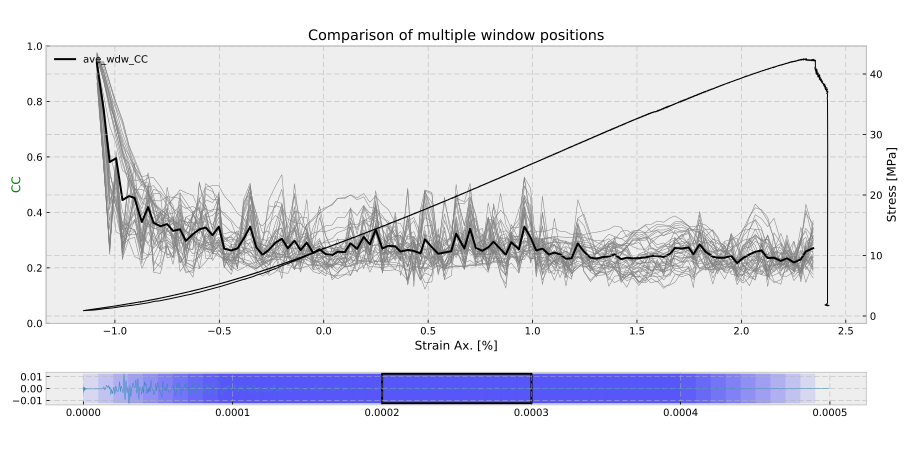
\includegraphics[width=150mm,scale=0.6]{Multi_wdw}
  \caption{The output image from the function displays multiple overlapping windows along with the average of all for a single lag value.}
\end{figure}

		%%%%%%%%%%%%%%
		\textbf{dispCWI\_pres(param, DB, TS, ccPlot\_list, PV\_full=None, PV1=None, PV2=None, PV3=None, PV4 = None, plot\_dic=\{\}):} \newline
		%%%%%%%%%%%%%%
        The flexible display of multiple input vectors\newline
        ---Inputs---
        param:       file summarising the processing run\newline
        DB:          Database of all PV and CC data to be plotted\newline
        TS:          Single TS in order to display the window positions\newline
        PV\_full    Non filtered PV\_data, used for plot if given\newline
        ccPlot\_list  List of tuples in CC data to plot \newline
        PV1=None     X-axis\newline
        PV2=None     Y2 right axis\newline
        PV3=None     Y3 right axis\newline
        plot\_dic    Dictionary to flexibility in ploting
        \newline
        
\begin{lstlisting}[basicstyle=\small, frame=single]
plot_dic = {'PV3_lb': 'Stress[MPa]', 'PV2_lb': 'Strain', 'CC_range': [0.95, 1],
		'X_axis_range': None, 'PV2_range': None, 
		'PV3_range': None, 'unit_m_4': 1000, 'elapsed_hours': True}
\end{lstlisting}

\begin{lstlisting}[basicstyle=\small, frame=single]
import dispCWI as disp
hdl = disp.dispUtilities.dispCWI_pres(param, PV_df, TScut_DB[3], ccPlot_list,
                                      None, PV1, PV2, PV3, PV4, plot_dic)
\end{lstlisting}

The output image from the function displays multiple overlapping windows along with the average of all for a single lag value.

\begin{figure}[hbt]
  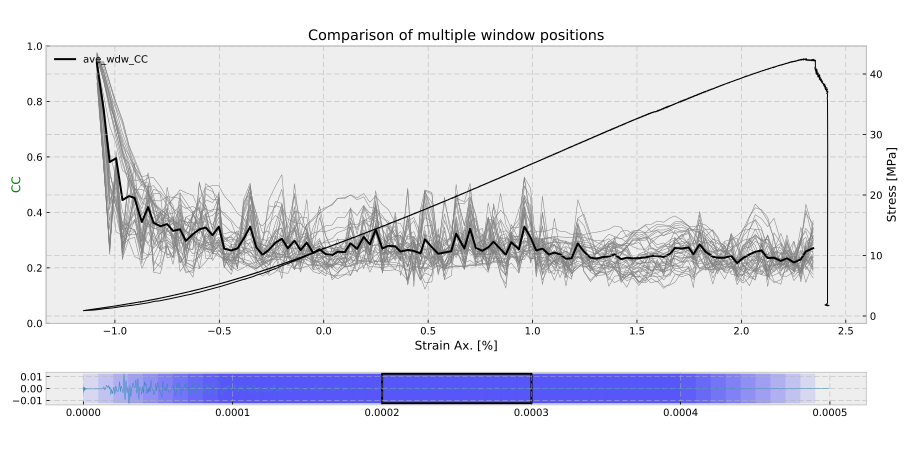
\includegraphics[width=150mm,scale=0.6]{Multi_wdw}
  \caption{The output image from the function displays multiple overlapping windows along with the average of all for a single lag value.}
\end{figure}

	%%%%%%%%%%%%%%%%%%%%%%%%%%%%%%%%%%%%%%%%%%%%%%
	\subsection{Module: pre\_process} 
	%%%%%%%%%%%%%%%%%%%%%%%%%%%%%%%%%%%%%%%%%%%%%%
	A collection of pre-processing utility functions.
		%%%%%%%%%%%%%%%%%%%%%%%%%%%%%%%%%%%%%%%%%%
		\subsubsection{Class: \texttt{utilities}:}
		%%%%%%%%%%%%%%%%%%%%%%%%%%%%%%%%%%%%%%%%%%
	\textbf{detect\_most\_linear(x, y, m):}\newline
        Finds the most linear portion of a line via the use of a covariance matrix\newline
        Inputs: \newline
        x: x-axis array of values\newline
        y: y-axis array of values\newline
        m: Length of most linear portion of line $(x, y)$\newline

        Outputs:\newline
        L\_end: \texttt{x\_end, y\_end} values at the end of the line\newline
        idx: Indices of the most linear portion of the line\newline

	%%%%%%%%%%%%%%%%%%%%%%%%%%%%%%%%%%%%%%%%%%%%%%
	\subsection{Module: postProcess} 
	%%%%%%%%%%%%%%%%%%%%%%%%%%%%%%%%%%%%%%%%%%%%%%
A collection of functions intended for post processing of CWI type data structures. For example, the calculation of Time Of Flight (TOF) velocity analysis can be added to a database through the use of the function \texttt{TS\_FBP}.
		%%%%%%%%%%%%%%%%%%%%%%%%%%%%%%%%%%%%%%%%%%
		\subsubsection{Class: \texttt{postProcess}:}
		%%%%%%%%%%%%%%%%%%%%%%%%%%%%%%%%%%%%%%%%%%
	Calls a sequence of functions which define the standard post processing. \newline
	
	\textbf{postProcess\_run(self):}
	Perform expected Post Processing. This function will perform First Break Picking, if the parameter FBP is given and set to True in the user input file.\newline
	
	\textbf{TS\_DB(self):}
	Convert TS matrix into a DataFrame with axis index in time.\newline
	
	\textbf{\_DatetimeIndex(self):}
	Check if the word Date is in the PV1 user defined parameter provided in the user input file. If so perform processing to provide pd.DatetimeIndex as the axis.\newline
	
	\textbf{\_stress\_strainP(self):}
	Perform stress strain calculation based on user defined inputs. Checks to see if input parameter \textit{stress\_strain} is given and is 'True' (string not boolian). Note this function assumes that the data frame contains the following columns:
	\begin{itemize}
		\item \texttt{LVDT1 and LVDT2}
		\item \texttt{Force(kN)}
	\end{itemize}
	
	\textbf{PV\_CC\_join(self):}
	Combine both PV and CC data into a single dataset based on.\newline
        measurement number
	%%%%%%%%%%%%%%%%%%%%%%%%%%%%%%%%%%%%%%%%%%%%%%
	\subsubsection{Class: \texttt{post\_utilities}:}
	%%%%%%%%%%%%%%%%%%%%%%%%%%%%%%%%%%%%%%%%%%%%%%MuM
	\textbf{\texttt{TS\_FBP}:}
	This function takes as input a pandas database of time series increasing columnweise, and performs analysis of the first break of energy on each trace. A window width of noise is defined, which is used to determine the expected standard deviation and mean of the noise for each trace. The function returns there outputs:
	
	\begin{itemize}
		\item \texttt{idx\_break}: The index of the first break detection point for each TS
	\end{itemize}

In order to check the first break picking, one can run the following.
\begin{lstlisting}[basicstyle=\small, frame=single]
import postProcess as pp
wdw_noise = 0.015 # in seconds
threshold = 0.5
verbose = True # request an interactive plot of the TS
mpd = 200
thdFactor = 10 # Factor added to stdThd*noiseStd for low noise environments
pp.post_utilities.TS_FBP(TS_DB, wdw_noise, threshold, thdFactor, mpd, verbose)
\end{lstlisting}

For further diagnostics one can run a trace by trace detection of peaks as follows:
\begin{lstlisting}[basicstyle=\small, frame=single]
import postProcess as pp
pp.post_utilities.detect_peaks(TScut_DB[7], mph=0.05, show=True)
\end{lstlisting}


%----------------------------------------------------------------------------------------
%	BIBLIOGRAPHY
%----------------------------------------------------------------------------------------

\bibliographystyle{apalike}

\bibliography{sample}

%----------------------------------------------------------------------------------------


\end{document}